% The flow chart created here depicts PyVVO's load modeling procedures.
\documentclass[tikz]{standalone}

\usepackage{amsmath}

% Load up the basic commands.
\usetikzlibrary{shapes.geometric, arrows.meta, fit, calc, positioning, automata, decorations.pathreplacing}

% Declare the layers
% https://tex.stackexchange.com/a/75498/208656
\pgfdeclarelayer{background}
\pgfsetlayers{background,main}

% tikzset for flowcharts.
% https://tex.stackexchange.com/a/342227/208656
% Reference for label shifting in style:
% https://tex.stackexchange.com/a/78690/208656
% Reference for curly braces:
% https://tex.stackexchange.com/a/20887/208656
\tikzset{flowchart/.style = {
	base/.style = {
		draw=black,
		very thick,
		inner sep=10pt,
		outer sep=0pt,
		text width=10.0cm,
		minimum height=0.8cm,
		align=flush center,
	},
	labelshift/.style = {
		prefix after command= {\pgfextra{\tikzset{every label/.style={xshift=0.42cm}}}}
	},
	startstop/.style = {
		base,
		labelshift,
		rectangle,
		rounded corners,
		fill=red!30
	},
	io/.style = {
		base,
		trapezium,
		trapezium left angle=70,
		trapezium right angle=110,
		trapezium stretches=true,
		fill=blue!30,
	},
	process/.style = {
		base,
		labelshift,
		rectangle,
		fill=orange!30
	},
	decision/.style = {
		base,
		text width=3.0cm,
		diamond,
		aspect=1.2,
		fill=green!30
	},
	arrows.meta/.style = {
		very thick,
	 	-{Stealth[]}
	},
	curlybrace/.style = {%
		draw=black,
		decorate,
		very thick,
		decoration={brace, amplitude=20pt, raise=6pt, mirror},
	},
	curlynode/.style = {
		draw=none,
		black,
		midway,
		xshift=2.75cm,
		text width=3cm	
	},
	backgroundbox/.style = {
		draw=none,
		inner sep=0.8cm,
		ultra thick,
		dashed,
		fill opacity=0.4
	}
}}

% Shortcut for inline code:
% https://stackoverflow.com/a/21344989
\newcommand{\code}[1]{\texttt{#1}}

% Label counter for the flow chart.
\newcounter{ac}
\renewcommand{\theac}{\alph{ac}}
\newcommand{\ac}[1]{(\refstepcounter{ac}\alph{ac})\label{#1}}

% To put parentheses around references:
\newcommand{\acref}[1]{(\ref{#1})}

% The following are for extracing coordinates.
% https://tex.stackexchange.com/a/33706/208656
\newdimen\XCoord
\newdimen\YCoord
\newcommand*{\ExtractCoordinate}[1]{\path (#1); \pgfgetlastxy{\XCoord}{\YCoord};}%
\newcommand*{\ExtractCoordinateTwo}[1]{\path (#1); \pgfgetlastxy{\XCoordTwo}{\YCoordTwo};}%

% Dimension and command for labeling boxes.
\newdimen\XLabel
\newcommand{\LabelNode}[1]{\ExtractCoordinate{$(#1.east)$}; \node (#1-label) at (\XLabel, \YCoord) {\ac{flow:#1}};}

\begin{document}
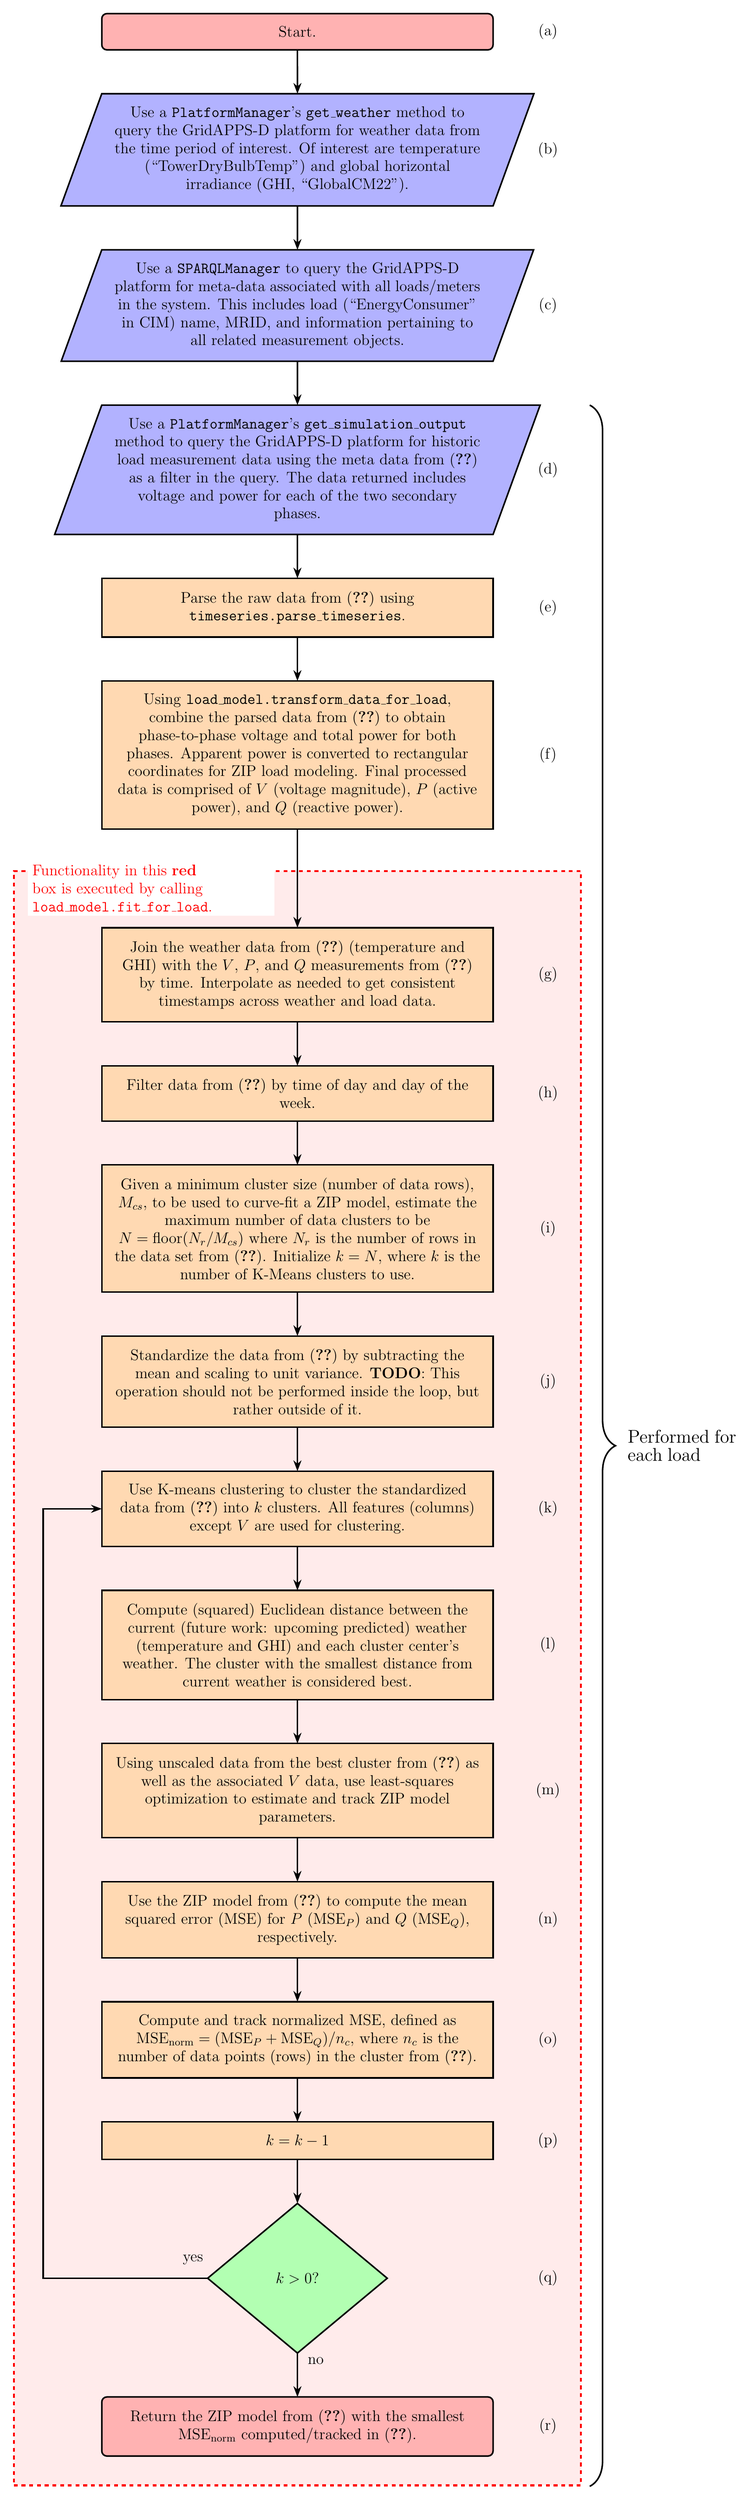
\begin{tikzpicture}[flowchart, node distance=1.2cm] 
\tikzstyle{every node}=[font=\large]

	%%%%%%%%%%%%%%%%%%%%%%%%%%%%%%%%%%%%%%%%%%%%%%%%%%%%%%%%%%%%%%%%
	% NODES
	%%%%%%%%%%%%%%%%%%%%%%%%%%%%%%%%%%%%%%%%%%%%%%%%%%%%%%%%%%%%%%%%
	\node (start)
	[startstop]
	{Start.};
	% Create a coordinate which will be referenced for all labels.
	\coordinate (start-east) at ($(start.east) + (1.5,0)$);
	\path ($(start-east)$); \pgfgetlastxy{\XLabel}{\YCoord};
	% Label our first node.
	\LabelNode{start}
	%
	\node (pull-weather-data)
	[io, below=of start]
	{Use a \code{PlatformManager}'s \code{get\_weather} method to query the GridAPPS-D
	platform for weather data from the time period of interest. Of interest are temperature
	(``TowerDryBulbTemp'') and global horizontal irradiance (GHI, ``GlobalCM22'').};
	\LabelNode{pull-weather-data}
	% 
	\node (pull-meta-data)
	[io, below=of pull-weather-data]
	{Use a \code{SPARQLManager} to query the GridAPPS-D platform for meta-data associated with
	all loads/meters in the system. This includes load (``EnergyConsumer'' in CIM) name, MRID, and
	information pertaining to all related measurement objects.};
	\LabelNode{pull-meta-data}
	%
	\node (pull-load-data)
	[io, below=of pull-meta-data]
	{Use a \code{PlatformManager}'s \code{get\_simulation\_output} method to query the
	GridAPPS-D platform for historic load measurement data using the meta data from
	\acref{flow:pull-meta-data} as a filter in the query. The data returned includes voltage
	and power for each of the two secondary phases.};
	\LabelNode{pull-load-data}
	%
	\node (parse-load-data)
	[process, below=of pull-load-data]
	{Parse the raw data from \acref{flow:pull-load-data} using \code{timeseries.parse\_timeseries}.};
	\LabelNode{parse-load-data};
	%
	\node (process-load-data)
	[process, below=of parse-load-data]
	{Using \code{load\_model.transform\_data\_for\_load}, combine the parsed data from
	\acref{flow:parse-load-data} to obtain phase-to-phase voltage and total power for both
	phases. Apparent power is converted to rectangular coordinates for ZIP load
	modeling. Final processed data is comprised of $V$ (voltage magnitude), $P$ (active power),
	and $Q$ (reactive power).};
	\LabelNode{process-load-data}
	% 
	\node (join-load-weather)
	[process, below=of process-load-data, yshift=-1.5cm]
	{Join the weather data from \acref{flow:pull-weather-data} (temperature and GHI)
	with the $V$, $P$, and $Q$ measurements from \acref{flow:process-load-data} by time.
	Interpolate as needed to get consistent timestamps across weather and load data.};
	\LabelNode{join-load-weather}
	%
	\node (time-filter)
	[process, below=of join-load-weather]
	{Filter data from \acref{flow:join-load-weather} by time of day and day of the week.};
	\LabelNode{time-filter}
	%
	\node (compute-max-clusters)
	[process, below=of time-filter]
	{Given a minimum cluster size (number of data rows), $M_{cs}$, to be used to curve-fit a
	ZIP model, estimate the maximum number of data clusters to be $N = \text{floor}(N_r / M_{cs})$
	where $N_r$ is the number of rows in the data set from \acref{flow:join-load-weather}. Initialize\
	$k = N$, where $k$ is the number of K-Means clusters to use.};
	\LabelNode{compute-max-clusters}
	%
	\node (standard-scale)
	[process, below=of compute-max-clusters]
	{Standardize the data from \acref{flow:join-load-weather} by subtracting the mean and scaling to
	unit variance. \textbf{TODO}: This operation should not be performed inside the loop, but 
	rather outside of it.};
	\LabelNode{standard-scale}
	%
	\node (cluster)
	[process, below=of standard-scale]
	{Use K-means clustering to cluster the standardized data from \acref{flow:standard-scale} into $k$
	clusters. All features (columns) except $V$ are used for clustering.};
	\LabelNode{cluster}
	%
	\node (select-cluster)
	[process, below=of cluster]
	{Compute (squared) Euclidean distance between the current (future work: upcoming predicted) 
	weather (temperature and GHI) and each cluster center's weather. The cluster with the smallest
	distance from current weather is considered best.};
	\LabelNode{select-cluster}
	%
	\node (ls-fit)
	[process, below=of select-cluster]
	{Using unscaled data from the best cluster from \acref{flow:select-cluster} as well as the associated $V$ data,
	use least-squares optimization to estimate and track ZIP model parameters.};
	\LabelNode{ls-fit}
	% 
	\node (mse)
	[process, below=of ls-fit]
	{Use the ZIP model from \acref{flow:ls-fit} to compute the mean squared error (MSE) for $P$
	($\text{MSE}_P$) and $Q$ ($\text{MSE}_Q$), respectively.};
	\LabelNode{mse}
	%
	\node (norm-mse)
	[process, below=of mse]
	{Compute and track normalized MSE, defined as
	$\text{MSE}_\text{norm} = (\text{MSE}_P + \text{MSE}_Q) / n_c$, where $n_c$ is the
	number of data points (rows) in the cluster from \acref{flow:select-cluster}.};
	\LabelNode{norm-mse}
	%
	\node (dec-k)
	[process, below=of norm-mse]
	{$k = k - 1$};
	\LabelNode{dec-k}
	%
	\node (k-gt-0)
	[decision, below=of dec-k, label={[yshift=+0.5cm] left:yes}, label={[xshift=+0.5cm] below:no}]
	{$k > 0$?};
	\LabelNode{k-gt-0}
	% 
	\node (select-model)
	[startstop, below=of k-gt-0]
	{Return the ZIP model from \acref{flow:ls-fit} with the smallest $\text{MSE}_\text{norm}$ 
	computed/tracked in \acref{flow:norm-mse}.};
	\LabelNode{select-model}
	
	%%%%%%%%%%%%%%%%%%%%%%%%%%%%%%%%%%%%%%%%%%%%%%%%%%%%%%%%%%%%%%%%
	% ARROWS
	%%%%%%%%%%%%%%%%%%%%%%%%%%%%%%%%%%%%%%%%%%%%%%%%%%%%%%%%%%%%%%%%
	\begin{pgfonlayer}{main}
	\draw[arrows.meta] (start) -- (pull-weather-data);
	\draw[arrows.meta] (pull-weather-data) -- (pull-meta-data);
	\draw[arrows.meta] (pull-meta-data) -- (pull-load-data);
	\draw[arrows.meta] (pull-load-data) -- (parse-load-data);
	\draw[arrows.meta] (parse-load-data) -- (process-load-data);
	\draw[arrows.meta] (process-load-data) -- (join-load-weather);
	\draw[arrows.meta] (join-load-weather) -- (time-filter);
	\draw[arrows.meta] (time-filter) -- (compute-max-clusters);
	\draw[arrows.meta] (compute-max-clusters) -- (standard-scale);
	\draw[arrows.meta] (standard-scale) -- (cluster);
	\draw[arrows.meta] (cluster) -- (select-cluster);
	\draw[arrows.meta] (select-cluster) -- (ls-fit);
	\draw[arrows.meta] (ls-fit) -- (mse);
	\draw[arrows.meta] (mse) -- (norm-mse);
	\draw[arrows.meta] (norm-mse) -- (dec-k);
	\draw[arrows.meta] (dec-k) -- (k-gt-0);
	\draw[arrows.meta] (k-gt-0) -- (select-model);
	\draw[arrows.meta] (k-gt-0.west) -| ++(-4.5,0) |- (cluster);
	% Extract/create coordinates for the upcoming optimization phase "fit" box.
	\coordinate (k-gt-0-west) at ($(k-gt-0.west) + (-4.5,0)$);
	\ExtractCoordinate{$(k-gt-0-west)$}
	\coordinate (k-gt-0-mirror) at (\XCoord * -1, \YCoord);

	\end{pgfonlayer}
	
	% Background layer.
	\begin{pgfonlayer}{background}
		% Place a coordinate above join-load-weather
		\coordinate (above-join-load-weather) at ($(join-load-weather.north) + (0.0cm, 0.75cm)$);
		% Draw a box around the procedures handled by load_model.fit_for_load.
		\node (fit-for-load)
		[backgroundbox, draw=red, fill=red!20, fit = (above-join-load-weather) (select-model) (k-gt-0-west) (k-gt-0-mirror)]
		{};
		\node (ffl-label)
		[yshift=-0.5cm, xshift=-4cm, red, fill=white, text width=6.5cm] at (fit-for-load.north) {Functionality in this \textbf{red} box is executed by calling \code{load\_model.fit\_for\_load}.}; 
	\end{pgfonlayer}
	
	% Curly brace. But we need some coordinates.
	\coordinate (curly-brace-top) at (fit-for-load.east |- pull-load-data.north east);
	\draw [curlybrace]
	(fit-for-load.south east) -- (curly-brace-top) node [curlynode] {\Large Performed for each load};
\end{tikzpicture}
\end{document}